\chapter{Apreciação das Técnicas Envolvidas\label{cap:fundamentacao}}

\section{Introdução}
  
  
  O desenvolvimento da solução proposta neste trabalho envolve o conhecimento de técnicas de controle de acesso e biometria, sistemas embarcados, projeto de circuitos eletrônicos, desenvolvimento de aplicações de rede e banco de dados. Esses conhecimentos são essenciais na execução do projeto apresentado no Capítulo 3, e contribuem para uma melhor compreensão do uso das ferramentas utilizadas em sua realização, portanto, são descritas neste capítulo as principais tecnologias presentes em cada uma das etapas de implementação do sistema proposto aqui.



\section{Controle de acesso}

  Controle de acesso é um termo usado em segurança física que refere-se a restrição seletiva de acesso. É a prática de permitir o acesso a uma propriedade, prédio, condomínio, sala ou qualquer local que tenha acesso restrito a pessoas autorizadas. O controle de acesso físico pode ser realizado por pessoas, um agente de segurança, porteiro ou recepcionista; por meios mecânicos como fechaduras e chaves; ou por meios tecnológicos, como sistemas eletrônicos baseados em autenticação, utilizando cartões, biometria ou senha. De acordo com a Associação das Indústrias de Segurança (\textit{Security Industry Association} -- SIA), controle de acesso é a utilização de dispositivos de qualificação ou métodos de identificação para controlar a entrada ou saída de pessoas em uma área ou estrutura \cite{privatesecurity}.

\nomenclature{SIA}{Associação das Indústrias de Segurança (\textit{Security Industry Association})}

  Honey \cite{electronicaccesscontrol} cita como a forma mais básica de controle de acesso eletrônico, um sistema doméstico, de baixa segurança, muito simples, destinado a proteger uma porta com fechadura. Nesse sistema, um visitante pode ser interrogado por uma comunicação interna, em um ponto local, através de um interfone simples. Ainda segundo Honey~\cite{electronicaccesscontrol}, o futuro do controle de acesso eletrônico seriam sistemas de alta segurança baseados em computadores inteligentes e multi-portas, com vigilância remota, mais fáceis de serem operados por usuários e práticos para visitantes, algo que já acontece na atualidade.


\subsection{Autenticação}
  
  
  Autenticação é o ato do usuário se identificar utilizando diversos mecanismos, como cartão, login e senha, biometria e token, por exemplo \cite{gerenciamentoid}, e pode ser utilizada para acesso lógico (computadores e sistemas) ou físico (catracas e portas). Além de ser um método de verificação da identidade de uma pessoa, a autenticação pode ser também um meio para atestar a procedência de um objeto.


\section{Biometria\label{secao:biometria}}

  Biometria é o estudo da mensuração de seres vivos, é a medida de características únicas de cada indivíduo, a partir da qual é possível identificá-lo \cite{handbookbiometrics}. Tais características podem ser físicas, como impressões digitais, geometria da palma, retina, íris, face, por exemplo; comportamentais, como assinatura manuscrita, voz, dinâmica de datilografia (digitação) e a forma como anda (caminhar); ou até mesmo química, como o odor corporal.  Dentre os métodos tecnológicos de controle de acesso, a biometria é a principal técnica empregada em aplicações de autenticação. Independente do tipo de biometria a ser utilizado no processo de verificação ou identificação, um sistema biométrico genérico é composto pelas seguintes etapas \cite{patel2008information, duffy2008handbook}:
  

\begin{itemize}
    \item Aquisição de dados
    
    O traço biométrico é lido por um sensor e a informação obtida é transformada em uma representação digital; como por exemplo uma imagem em níveis de cinza capturada na leitura de uma impressão digital, ou uma amostra de saliva, no caso do DNA.
    
    \item Extração de características
    
   
    De acordo com o tipo de biometria, são extraídas de um dado biométrico somente as informações úteis, isto é, aquelas que representam características de identificação de um indivíduo. Desta forma, ocorre a redução do conjunto de medidas biométricas de um indivíduo, resultando em um volume menor de dados que é transformado em um modelo (\textit{template}).
    

    \item Armazenamento
    
    O \textit{template} é armazenado em uma memória ou banco de dados e fica disponível para as operações de verificação ou identificação.
    
    \item Comparação
    
    Nessa etapa é gerado um modelo temporário para a autenticação ou identificação de um indivíduo. Esse modelo é comparado com o 
    \textit{template} de um usuário específico ou com todos os \textit{templates} registrados. 
    
\end{itemize}


  A biometria é um método de autenticação se destaca dentre as demais, devido ser uma técnica baseada em características individuais que não podem ser roubadas, emprestadas ou esquecidas e até mesmo são difíceis de serem forjadas. No entanto, qualquer característica física ou comportamental somente pode ser considerada como um identificador biométrico, para o reconhecimento de indivíduos, se ela satisfizer aos seguintes critérios \cite{maltoni2009handbook}:

\begin{itemize}
    
\item Universalidade

  Todos os indivíduos de uma população a ser estudada devem possuir a característica analisada.

\item Unicidade ou Singularidade

  Uma característica biométrica deve ser única para cada indivíduo ou apresentar possibilidade nula/desprezível de pessoas distintas possuírem características idênticas.

\item Permanência

  A característica deve ser imutável. Devido ao envelhecimento, existem alterações que implicam em mudanças nas condições de saúde ou emocionais, além de possíveis alterações nas condições do ambiente de coleta, que podem modificar a característica analisada.Dessa forma, a característica avaliada deve ser invariante ao longo do tempo a ponto de não comprometer os critérios de identificação do indivíduo.

\item Coletabilidade

  A característica a ser analisada deve permitir ser mensurada quantitativamente. Além disso, a coleta deve também permitir processamento para a extração das informações desejadas. Na prática, existem outros aspectos que devem ser considerados, como performance, aceitabilidade e evasão.

\end{itemize}

Além dos critérios mínimos para que qualquer característica física ou comportamental seja considerada como um identificador biométrico, existem outros fatores que podem ser analisados para avaliar dado um tipo de biometria, como por exemplo:


\begin{itemize}
    
    \item Performance
    
    refere-se à precisão do reconhecimento, velocidade, robustez, os recursos necessários para alcançar a precisão de reconhecimento desejado e velocidade, assim como fatores operacionais ou ambientais que afetam a precisão de reconhecimento e velocidade;


    \item Aceitabilidade
    
    Indica o grau de aceitação de uma tecnologia biométrica. Desta forma, esse critério aponta se as pessoas estão dispostas a aceitar o uso de um determinado identificador biométrico;
    
    \item Evasão
    
    A evasão é um critério que avalia o grau de vulnerabilidade de um sistema, isto é, qual a facilidade do sistema ser enganado através do uso de métodos fraudulentos.
    
\end{itemize}



\subsection{Tipos de biometria\label{secao:tiposdebiometria}}
Nesta seção são descritos os principais tipos de biometria encontrados na literatura.


\begin{itemize}
    
\item Face

  A face é um dos tipos de biometria mais aceitável, pois é um método não invasivo e comum no reconhecimento usado pelos humanos em interações visuais. Normalmente há resistência ao  uso de coletas de dados biométricos invasivas, pois elas exige o contato físico do usuário com os dispositivos de coleta e tendem a se tornar desagradáveis para o ser humano.
  
  O desenvolvimento de técnicas de reconhecimento de face eficientes torna-se difícil devido aos efeitos de envelhecimento, expressão facial, variações no ambiente de captura da imagem e na posição da face em relação à câmera, e outros aspectos relativos as variações das características da face que devem ser considerados \cite{maltoni2009handbook}.


\item Termografia

  O padrão de radiação de calor do corpo humano é uma característica individual que pode ser capturada por uma câmera infravermelho de forma discreta e que gera imagens muito semelhantes a fotografia comum (espectro visível). Os sistemas baseados em termografia são não invasivos, portanto, não há o contato entre o indivíduo e o instrumento de reconhecimento. No entanto, ambientes de temperatura não controlada desafiam o sensoreamento, pois comprometem a fase de aquisição de imagens que é afetada pelas alterações drásticas de calor oriundas do ambiente em que o copro se encontra, devido as interferências de aquecedores, escapamento de veículos, e ar-condicionados \cite{maltoni2009handbook}.


\item Andar

  O reconhecimento através da caracterização do andar de um indivíduo é complexo tanto no aspecto temporal quanto espacial. A característica do andar de uma pessoa não é tão distinta quanto a de outra, mas é suficientemente característica para permitir a identificação em aplicações de baixa segurança. Essa é uma característica que sofre alterações de acordo com o cansaço, peso corporal, ferimentos e lesões envolvendo articulações e cérebro, ou devido a embriagues\cite{maltoni2009handbook}.


\item Geometria da mão e do dedo

  O reconhecimento por geometria da mão e do dedo é baseado em características peculiares, como a forma, tamanho, comprimento e largura. Os sistemas que utilizam esse método de reconhecimento dependem da cooperação da pessoa a ser identificada para a aquisição de imagens frontal e lateral da palma da mão. O desenvolvimento de aplicações baseadas nesse tipo de biometria é atrativo para sistemas de memória e largura de banda limitados \cite{maltoni2009handbook}, devido aos requisitos de representação da mão e do dedo serem muito pequenos.


\item Dinâmica de digitação

  A dinâmica de digitação é baseada na suposição de que cada pessoa digite de uma forma característica, sendo considerada uma característica comportamental de baixo fator de unicidade, assim como o andar, mas que oferece informações discriminatórias suficientes para a verificação de identidade. Os sistemas de reconhecimento por dinâmica de digitação fazem o monitoramento discreto de como uma pessoa digita, podendo analisar os seguintes aspectos \cite{ilonen2003keystroke}: intervalo de tempo entre o pressionamento de teclas consecutivas; tempo que uma tecla fica pressionada; tempo total da digitação; frequência da digitação de teclas erradas; e o hábito de usar teclas diferentes do teclado. Essa técnica tem um custo mais baixo em relação à outras técnicas de biometria, devido não necessitar de um equipamento dedicado ao monitoramento, e pode ser aplicada em sistemas de média segurança.  

\item Íris

  A imagem da íris normalmente é capturada através de um processo que não exige contato físico, mas depende da cooperação do usuário, para assegurar que a íris está a uma distância predeterminada do plano focal da câmera. Os leitores de íris colhem dados exatamente da porção colorida do olho a uma distância de 25 cm, em média, e faz uma leitura em menos de vinte segundos \cite{gerenciamentoid}. A tecnologia de reconhecimento da íris é uma técnica precisa e rápida \cite{maltoni2009handbook}, é uma das melhores opções de autenticação e também uma das mais caras \cite{gerenciamentoid}.

\item Retina

  A identificação por retina envolve a análise da camada de vasos sanguíneos presentes no fundo dos olhos. Essa técnica usa uma fonte de luz de baixa intensidade por meio de um acoplador óptico para verificar as características individuais da retina. O Escaneamento de retina pode ser bastante preciso, mas exige que o usuário olhe para um determinado ponto no leitor e se concentre, desta forma, há o contato próximo com o dispositivo e isso pode ser desconfortável para alguns usuários \cite{liu2001practical}. 


\item Assinatura

  A maneira como uma pessoa assina seu nome é considerada uma característica individual \cite{maltoni2009handbook} e a técnica de verificação de assinatura se apropria de características importantes, como a velocidade de escrita, rapidez, pressão e forma da finalização da assinatura \cite{liu2001practical}, para realizar a autenticação de usuários. A assinatura é uma característica comportamental que muda ao longo de um período de tempo e são influenciadas pelas condições físicas e emocionais do signatário.


\item Voz

  A voz pode ser utilizada como um identificador biométrico, pois o som sintetizado pela fala humana possui características individuais resultantes de aspectos físicos da boca, nariz, lábios e trato vocal; e comportamentais, como pronuncia e a maneira da falar (sotaque); sendo considerada uma forma de biometria comportamental \cite{clarke2011transparent}. 

  Além disso, vale ressaltar que, apesar de similar, um sistema de reconhecimento de voz é diferente de um sistema de identificação de voz. O primeiro é o processo que reconhece \textit{o quê} uma pessoa fala. Enquanto o segundo, sistema de identificação de voz, reconhece \textit{quem} está falando \cite{clarke2011transparent}. A verificação de voz é uma técnica não invasiva e pode operar de modo estático (texto-dependente), no qual o sistema deve identificar um usuário a partir da pronuncia de um texto fixo pré-determinado; ou de modo dinâmico (texto-independente), no qual o sistema deve identificar um usuário independente da fala.


\item Orelha
    
  As orelhas possuem poucas características para descrevê-las.No entanto, a sua estrutura é única, e por isso pode ser usada como fator biométrico para identificação passiva. Diversas abordagens de reconhecimento biométrico da orelha podem ser encontradas na literatura \cite{reconhecimentoorelha, pflug2012ear, yan2006automatic, yuan2007ear, zhang2005novel, chang2003comparison}.

\item Odor

  É um tipo de biometria comportamental, pouco usado, baseado no sentido do olfato \cite{revett2008behavioral}. Cada individuo humano carrega consigo um cheiro particular produzido por substâncias químicas voláteis. Essa característica pode ser convertida em um modelo individual usado por sensores químicos capazes de capturar o odor corporal de forma não intrusiva, através de partes específicas do corpo, como a mão \cite{vacca2007biometric}.



\end{itemize}


\subsection{Comparação entre os tipos de biometria}

  Os identificadores biométricos são empregados em diversas aplicações e cada um deles tem suas vantagens e desvantagens. Assim, a escolha de uma técnica de biometria depende da aplicação e de suas características, bem como, os requisitos operacionais e estruturais. Os identificadores também podem ser comparados de acordo com os requisitos citados na Seção~\ref{secao:biometria} (universalidade, singularidade, permanência etc), como mostrado na Tabela~\ref{tecnicasbio}, a partir da qual, nota-se que a impressão digital apresenta um balanço nos níveis das propriedades desejadas.


\begin{table}[!b]
\centering
\caption{Comparação de tecnologias de biometria. Alto, Médio e Baixo são indicados por A, M e B, respectivamente}
\label{tecnicasbio}
\begin{tabular}{|c|m{0.3cm}|m{0.3cm}|m{0.3cm}|m{0.3cm}|m{0.3cm}|m{0.3cm}|m{0.3cm}|m{0.3cm}|}
\hline
\rowcolor[HTML]{9B9B9B}
\textbf{Identificador Biométrico} & 
\rotatebox{90}{\textbf{Universalidade }} & 
\rotatebox{90}{\textbf{Singularidade }} & 
\rotatebox{90}{\textbf{Permanência }} & 
\rotatebox{90}{\textbf{Coletabilidade }} & 
\rotatebox{90}{\textbf{Performance }} & 
\rotatebox{90}{\textbf{Aceitabilidade }} & 
\rotatebox{90}{\textbf{Evasão }} \\ \hline
DNA                                       & A & A & A & B & A & B & B \\ \hline
Orelha                                    & M & M & A & M & M & A & M \\ \hline
Face                                      & A & B & M & A & B & A & A \\ \hline
Termografia facial                        & A & A & B & A & M & A & B \\ \hline
\rowcolor[HTML]{C0C0C0} Impressão digital & M & A & A & M & A & M & M \\ \hline
Andar                                     & M & B & B & A & B & A & M \\ \hline
Geometria da mão                          & M & M & M & A & M & M & M \\ \hline
Veias da palma da mão                     & M & M & M & M & M & M & L \\ \hline
Íris                                      & A & A & A & M & A & B & B \\ \hline
Digitação                                 & B & B & B & M & B & M & M \\ \hline
Odor                                      & A & A & A & B & B & M & B \\ \hline
Retina                                    & A & A & M & B & A & B & B \\ \hline
Assinatura                                & B & B & B & A & B & A & A \\ \hline
Voz                                       & M & B & B & M & B & A & A \\ \hline        
\end{tabular}
\vspace{5mm}

Fonte: Adaptado de \cite{maltoni2009handbook}.\\


\end{table}


\subsection{Impressão Digital}

  A impressão digital é a tecnologia de biometria mais utilizada~\cite{bosworth2014computer}. Além disso, ela é uma das técnicas mais explorada na literatura e apresenta custos de implantação relativamente \\baixos comparados a outras tecnologias, como as citadas na Seção~\ref{secao:tiposdebiometria}. Essas e outras vantagens justificam a popularização do uso desse tipo de biometria, que se mantém  entre as mais utilizadas, conforme mostra o gráfico comparativo da Figura~\ref{mercado_bio}, que representa a distribuição do mercado por tecnologia biométrica.


  \begin{figure}[ht]
  \begin{center}
  \caption{Distribuição de mercado por tecnologia biométrica}
  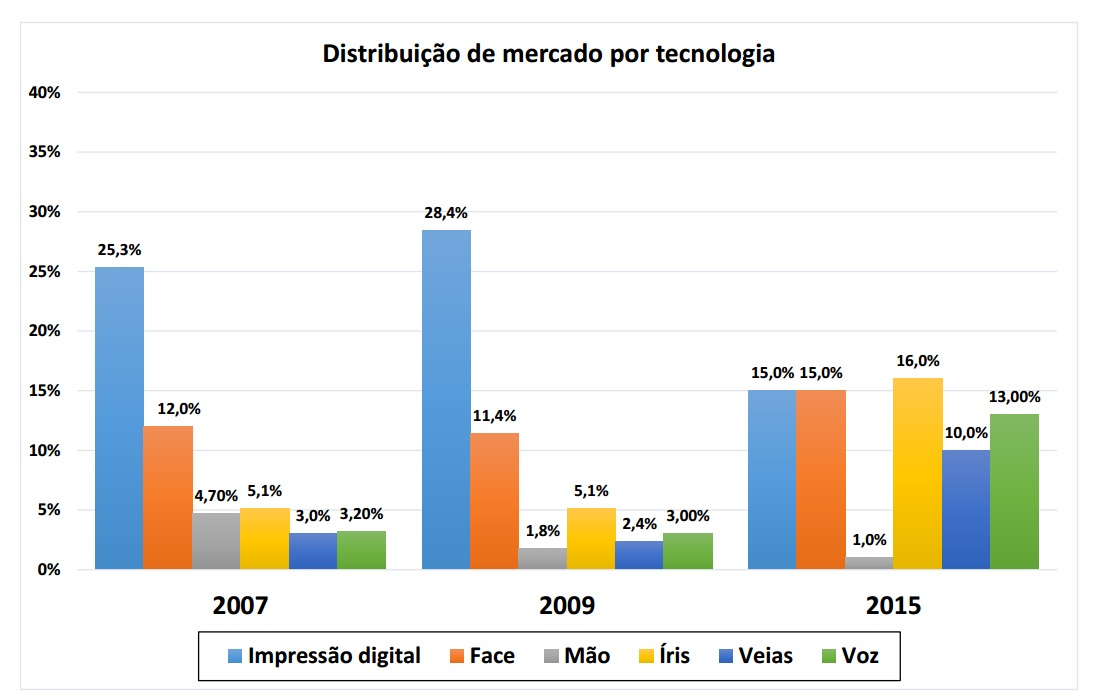
\includegraphics[scale=0.55]{figuras/cap2/mercado_bio.jpg}\\
  Fonte: Grupo de Biometria Internacional \textit{(\textit{Internacional Biometric Group$^{\copyright}$} -- IBG)} \cite{larsen2008biometric, zhang20133d, bosworth2014computer}.
  \label{mercado_bio}
  \end{center}
  \end{figure}

\nomenclature{IBG}{Grupo de Biometria Internacional (\textit{Internacional Biometric Group$^{\copyright}$})}


 Uma das desvantagens das técnicas de impressão digital é a possibilidade de fraudes. Por ser uma das tecnologias de biometria mais conhecidas \cite{bosworth2014computer}, há muitas informações sobre essa técnica disponível ao público. Apesar de não ser um processo simples, existe a possibilidade de falsificação de digital, utilizando um dedo falso produzido com látex ou outro material; ou até mesmo, em casos extremos, utilizando um dedo real amputado, pois a maioria dos leitores de impressões digitais não tem a capacidade de discriminação entre um tecido vivo e um morto. É indiscutível o fato de que a criminalidade corre contra os avanços da tecnologia, principalmente quando se trata de segurança. Portanto, é necessário conhecer as vulnerabilidades da técnica a ser utilizada para adotar medidas de correção de erros e prevenção de falhas para evitar possíveis fraudes e ataques. Outro problema enfrentado na implantação de sistemas de impressão digital para autenticação é a aceitação por parte dos usuários. Muitas pessoas não gostam de inserir o dedo no dispositivo de leitura. Outras pessoas, com receio de que o dado seja utilizado para outros fins, não aceitam a utilização do sistema por associarem a técnica à aplicações relacionadas a perícias forense, investigações criminais e a execução da lei \cite{bosworth2014computer, maltoni2009handbook}.


\subsubsection{Formação das impressões digitais}
 As impressões digitais são formadas nos sete primeiros meses de desenvolvimento do feto e não se alteram ao longo da vida do indivíduo, a não ser por motivos excepcionais, como acidentes, queimaduras ou cortes, ainda assim, tem a capacidade de se regenerar. A impressão digital ou datilograma é a reprodução do desenho digital resultante da combinação de cristas papilares e sulcos interpapilares localizados na polpa digital \cite{tavares1991papiloscopia}. As cristas papilares são os relevos epidérmicos situados na palma das mãos e na planta dos pés. Elas são separadas por depressões chamadas de sulcos interpapilares, formando assim os desenhos papilares \cite{couto2009segredos, holder2011fingerprint}, inclusive da superfície do tecido carnoso dos dedos (polpa digital)

\subsubsection{Leitura de impressão digital}
  A captura de impressão digital, bem como as técnicas e os equipamentos empregados, para fins de investigações criminais ou perícias forenses, são diferentes daqueles utilizados para fins de controle de acesso, que normalmente são mais amigáveis, mais compactos e mais baratos \cite{maltoni2009handbook}.

  Para fins de controle de acesso, as aplicações que envolvem a leitura da impressão digital podem empregar diferentes tipos de sensores que fazem a captura direta da imagem do dedo. Sem o uso de sensores específicos para a aquisição de imagens digitais dos dedos, a obtenção da imagem da digital pode ser feita por aquisição \textit{off-line}, em que ocorre a digitalização de uma imagem da impressão digital gravada em  papel.  Nesse processo, a superfície do dedo do usuário que contém o desenho digital é coberto de tinta e em seguida o dedo é pressionado contra um cartão de papel. A imagem impressa no cartão é digitalizada por um \textit{scanner}, que produz a imagem digital final que é utilizada no processo de identificação. Esse era o principal método usado por Sistemas de Identificação de Impressão Digital Automatizados (\textit{Automated Fingerprint Identification System} -- AFIS) antes do surgimento de sensores especializados. No entanto, esse processo é demorado para aplicações de controle de acesso. Assim, é necessário o uso de sensores específicos para a leitura de impressões digitais em tempo real, pois eles realizam o processo de digitalização em uma única etapa e agem mais rápido na leitura para reprodução da imagem digital. A Figura~\ref{leitor_bio} mostra o diagrama de um sistema eletrônico de leitura de impressão digital.

\nomenclature{AFIS}{Sistema de Identificação de Impressão Digital Automatizado (\textit{Automated Fingerprint Identification System})}


  Na Figura~\ref{leitor_bio}, o leitor representa o módulo interno ao aparelho, responsável por capturar a imagem da superfície do dedo. Essa imagem é convertida de analógica para um padrão digital. A imagem digital gerada na conversão A/D é enviada para um dispositivo externo, geralmente um computador, através de uma interface de comunicação responsável também pela troca de outras informações com o dispositivo. 
  
  
  Atualmente existem diversos tipos de sensores, mas quase todos são baseados em tecnologia ótica,  estado sólido ou ultrassom. Assim, a imagem adquirida por cada um desses sensores pode gerar diferentes resultados, conforme mostrado no exemplo da Figura~\ref{tipos_sensores}.


  \begin{figure}[!b]
  \begin{center}
  \caption{Diagrama de blocos de um sistema eletrônico de leitura de impressão digital.}
  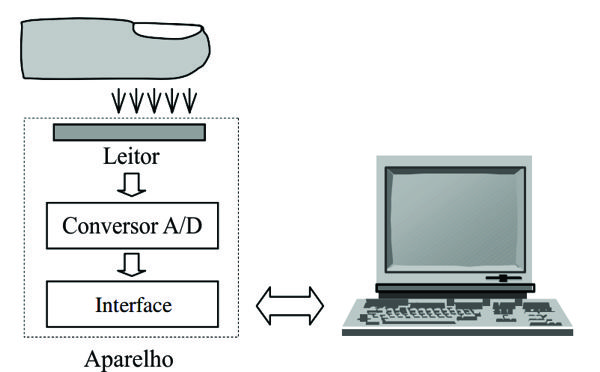
\includegraphics[scale=0.6]{figuras/cap2/leitor_bio.jpg}\\
  Fonte: Adaptado de \cite{maltoni2009handbook}.
  \label{leitor_bio}
  \end{center}
  \end{figure}


  \begin{figure}[!t]
  \begin{center}
  \caption{Imagens de impressão digital: a) sensor óptico; b) sensor capacitivo; c) sensor piezoelétrico; d) sensor térmico.}
  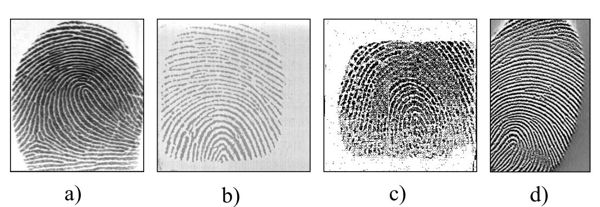
\includegraphics[scale=0.75]{figuras/cap2/tipos_sensores.jpg}\\
  Fonte: Adaptado de \cite{maltoni2009handbook}.
  \label{tipos_sensores}
  \end{center}
  \end{figure}


\subsubsection{Extração de características}
  A imagem da impressão digital é formada pela disposição de cristas (linhas escuras) e vales (linhas claras), como mostra a Figura~\ref{cristas_vales}. Através dessa disposição, é possível gerar um modelo de características para a identificação de usuários. Essas características são extraídas a partir do reconhecimento de terminações ou bifurcações de saliências, chamadas de \textit{minúcias}, e de outros elementos, como \textit{delta} e \textit{núcleo}, ilustrados na Figura~\ref{nucleo}, que são denominados \textit{regiões singulares}. O \textit{delta} é o ângulo ou triângulo formado pelas cristas papilares; e o \textit{núcleo} é um ponto central localizado na polpa da digital e pode ser também definido como um \textit{laço} [veja as Figuras~\ref{regioes_singulares}(a) e ~\ref{regioes_singulares}(b)] ou \textit{espiral} [mostrado na Figura~\ref{regioes_singulares}(c)]. Quando a digital não contém um laço ou espiral é difícil definir um núcleo. Desta forma, em alguns casos a região pode ser classificada como \textit{arco} (Figura~\ref{regioes_singulares} - d).  Além de bifurcações e terminações existem outros tipo de minúcias, na Tabela~\ref{tipos_minucias} são listados os tipos mais comuns de minúcias.



  \begin{figure}[!ht]
  \begin{center}
  \caption{Cristas e vales em uma imagem de impressão digital.}
  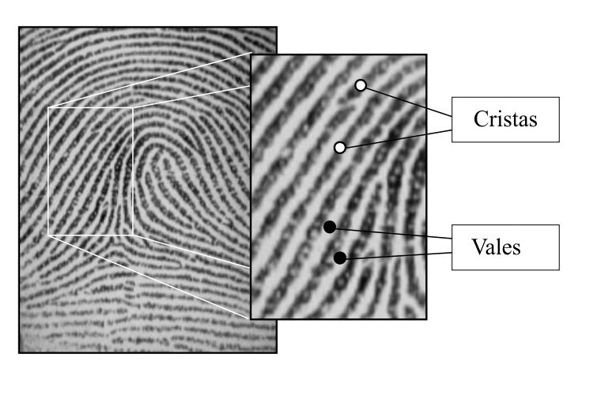
\includegraphics[scale=0.6]{figuras/cap2/cristas_vales.jpg}\\
  Fonte: Adaptado de \cite{maltoni2009handbook}.
  \label{cristas_vales}
  \end{center}
  \end{figure}
  
 
  \begin{figure}[!ht]
  \begin{center}
  \caption{Núcleo e delta em um imagem de impressão digital.}
  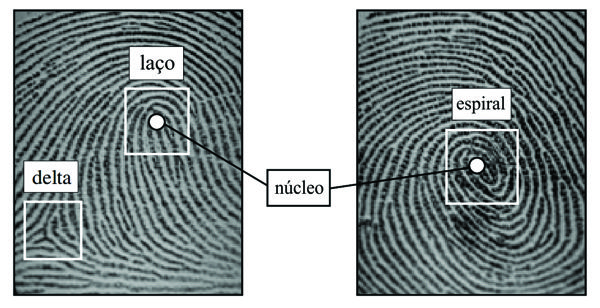
\includegraphics[scale=0.7]{figuras/cap2/nucleo.jpg}\\
  Fonte: Adaptado de \cite{maltoni2009handbook}.
  \label{nucleo}
  \end{center}
  \end{figure}
 
  \begin{figure}[!ht]
  \begin{center}
  \caption{Impressões digitais caracterizada por por \textit{laço} à esquerda e à direita, \textit{espiral} e \textit{arco}.}
  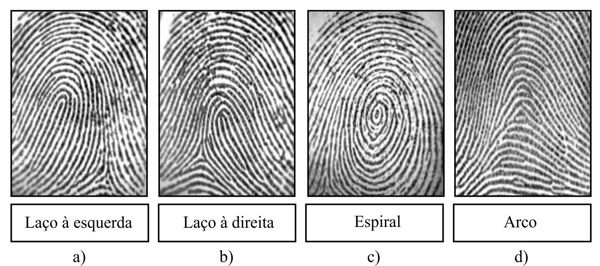
\includegraphics[scale=0.8]{figuras/cap2/regioes_singulares.jpg}\\
  Fonte: Adaptado de \cite{maltoni2009handbook}.
  \label{regioes_singulares}
  \end{center}
  \end{figure}
  
  
  \begin{table}[]
  \centering
  \caption{Os tipos mais comuns de minúcias.}
  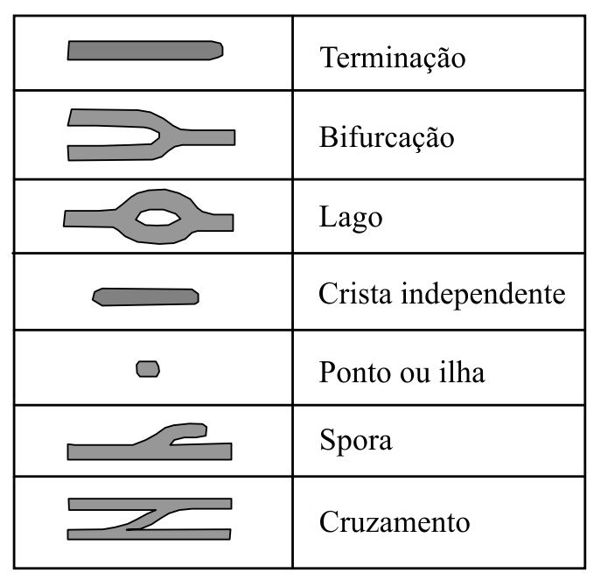
\includegraphics[scale=0.54]{figuras/cap2/tipos_minucias.jpg}\\
  Fonte: Adaptado de \cite{maltoni2009handbook}.
  \label{tipos_minucias}
  \end{table}
  
  
  A partir do uso das características citadas, existem várias técnicas e algoritmos desenvolvidos para o processamento e reconhecimento de impressões digitais na literatura biométrica \cite{bhanu2012computational, sarfraz2005computer, ratha2007automatic, alonso2007comparative, tico2001fingerprint, calabaide2006biometria}. Isso inclui, necessariamente, o uso de diferentes técnicas de processamento de imagens para extração de características e geração de modelo para comparação de usuários nos processos de verificação e autenticação. As abordagens de reconhecimento de digitais são basicamente divididas em três categorias \cite{maltoni2009handbook}: 
  
  \begin{itemize}
  \item Baseado em correlação
      
  Duas imagens de impressões digitais, no nível de tons de cinza, são sobrepostas e a correlação entre os \textit{pixels} correspondentes é computada mediante diferentes alinhamentos, deslocamentos e rotações.

  \item Baseado em minúcias
  
  \textit{Minúcias} são extraídas de duas impressões digitais e armazenadas como conjuntos de pontos no plano bidimensional (\textit{template}). O reconhecimento baseado em \textit{minúcias} consiste essencialmente de encontrar o alinhamento entre o modelo armazenado e o modelo a ser comparado. Isso resulta em um número máximo de \textit{minúcias} semelhantes.


  \item Baseado em cristas
 
  A extração de \textit{minúcias} é difícil em imagens de impressão digital de baixa qualidade, mas existem outras características do padrão de crista da digital, como orientação local, frequência, forma e informações de textura, podem ser extraídas com mais segurança que as \textit{minúcias}, mesmo que a distinção dessas características de crista sejam inferiores.

  \end{itemize}
  
  
  Portanto, qualquer técnica de reconhecimento de impressão digital gera o seu modelo de características baseada em uma dessas abordagens para a comparação de digitais.
  


\subsubsection{Sistemas biométricos}

  Dependendo do contexto da aplicação, todo sistema biométrico pode ser classificado de forma geral, como um \textit{sistema de identificação} ou \textit{sistema de  autenticação}, e ambos dispõe de três modos essenciais de operação: 

\begin{itemize}
     

\item Registro

  No registro é obtido o dado biométrico. Nesse processo é criado um modelo (\textit{template}), a partir da extração da característica biométrica do usuário. Cada usuário recebe um número de identificação pessoal(\textit {Personal Identification Number} -- PIN), que é vinculado ao seu modelo biométrico 
  armazenado no banco de dados, para posterior comparação nas operações de verificação (autenticação) e identificação. Na Figura~\ref{registro}, tem-se o diagrama da operação de registro. 

\nomenclature{PIN}{Número de identificação pessoal  (\textit{Personal Identification Number})}

 \begin{figure}[!ht]
  \begin{center}
  \caption{Sistema biométrico: registro.}
  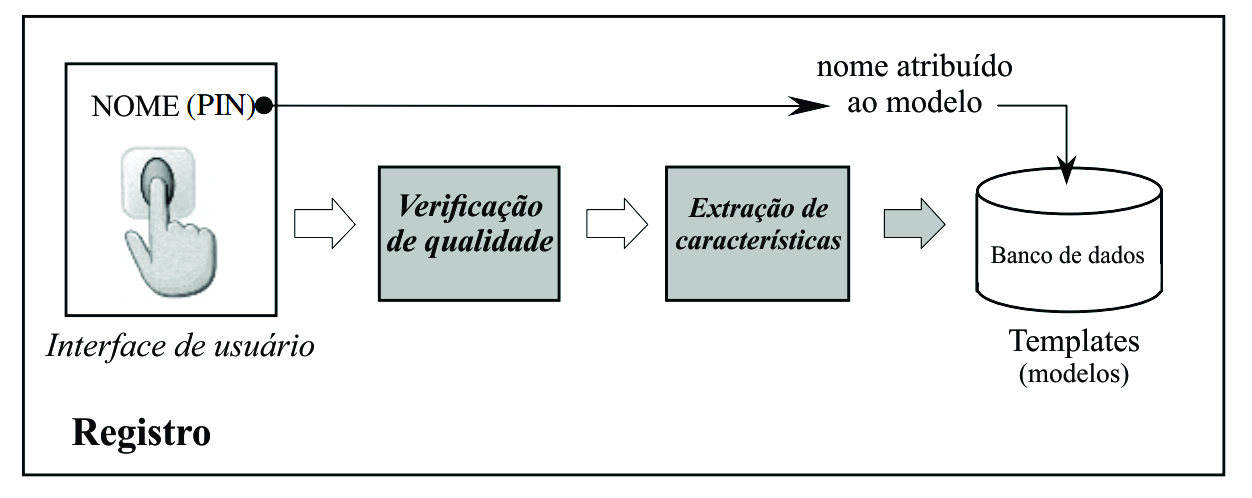
\includegraphics[scale=0.45]{figuras/cap2/registro.jpg}\\
  Fonte: Adaptado de \cite{maltoni2009handbook}.
  \label{registro}
  \end{center}
  \end{figure}
 


\item Verificação ou autenticação 

  No processo de verificação, também conhecido como autenticação, a característica biométrica do usuário que tenta autenticar-se é coletada e comparada a um único modelo. No entanto, não trata-se de qualquer modelo, pois o \textit{template} gerado na leitura é comparado especificamente com o modelo, no banco de dados, que possui o PIN informado informado pelo usuário. A Figura~\ref{verificacao} ilustra o diagrama dessa operação. 

 \begin{figure}[!ht]
  \begin{center}
  \caption{Sistema biométrico: verificação.}
  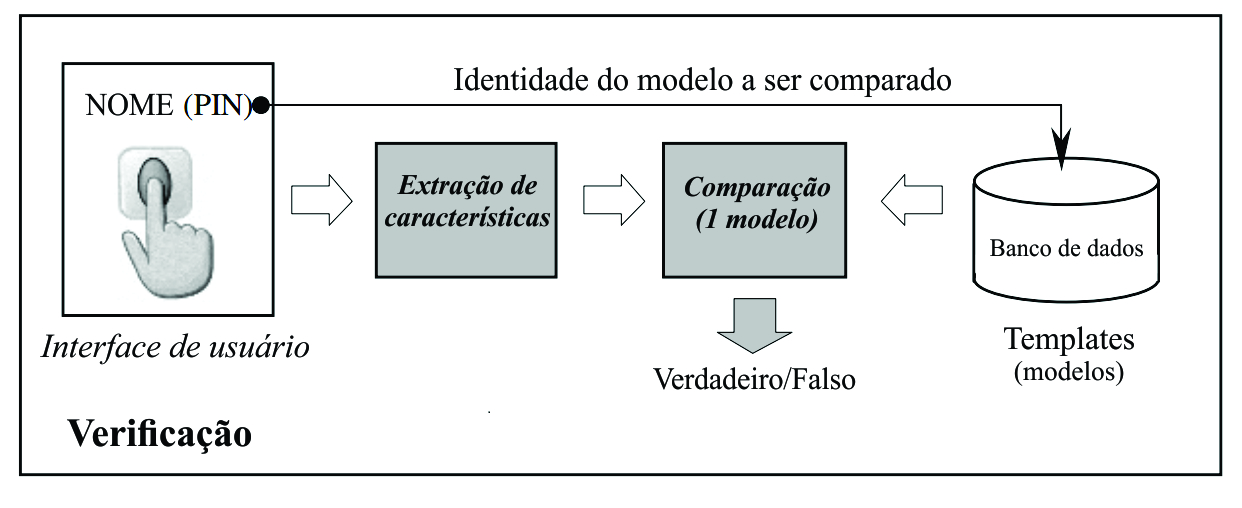
\includegraphics[scale=0.45]{figuras/cap2/verificacao.jpg}\\
  Fonte: Adaptado de \cite{maltoni2009handbook}.
  \label{verificacao}
  \end{center}
  \end{figure}

\item Identificação

  A identificação é um processo que compara a característica biométrica do usuário a ser identificado, com a característica biométricas de todos os usuários cadastrados no banco de dados. Por isso, é um processo custoso em termos de processamento. Essa operação requer que o dado biométrico de um determinado usuário seja lido e comparado a todos os modelos armazenados no banco de dados, a fim de obter como resultado um conjunto de possíveis usuários, uma lista com as identificações que apresentarem maior similaridade em relação as características do usuário em questão. O diagrama desse processo é mostrado na Figura~\ref{identificacao}

 \begin{figure}[!ht]
  \begin{center}
  \caption{Sistema biométrico: identificação.}
  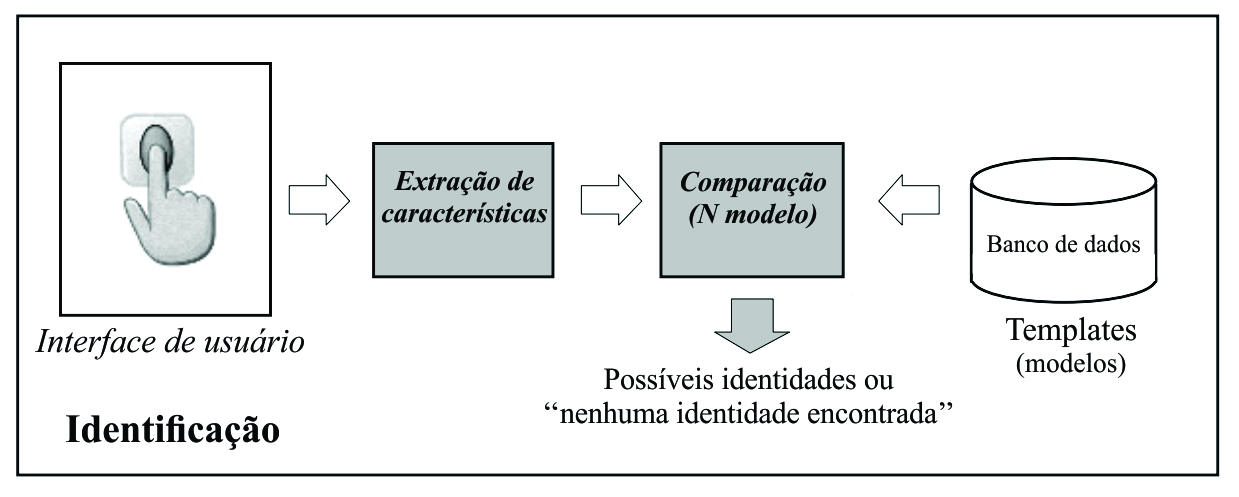
\includegraphics[scale=0.45]{figuras/cap2/identificacao.jpg}\\
  Fonte: Adaptado de \cite{maltoni2009handbook}.
  \label{identificacao}
  \end{center}
  \end{figure}

\end{itemize}



\section{Arduino}

   O Arduino é uma plataforma de \textit{hardware} \textit{open source}, ideal para a criação de dispositivos de entrada e saída que permitam interação com o ambiente \cite{arduino}, possui sua própria interface de programação e utiliza uma linguagem de alto nível, tornando fácil a sua utilização para desenvolvedores. Tal plataforma utiliza uma camada simples de \textit{software} implementada no \textit{hardware}, o \textit{bootloader}, e uma interface de fácil usabilidade para programação. O processamento do \textit{hardware} é realizado por microcontroladores e cada versão da placa apresenta um microcontrolador diferente. Normalmente é necessário utilizar um dispositivo específico para programar um microcontrolador. No entanto, essa programação é possível através da instalação de um sistema de instruções operacionais (\textit{firmware} ou \textit{bootloader}) no microcontrolador, que permite a instalação (programação) de novas instruções através de um programador externo (interface de computador) \cite{arduinocc_bootloader}. A interface de programação da placa utiliza a linguagem \textit{Processing}, a qual é baseada na linguagem C/C++ e também é \textit{open source}. Através do bootloader dispensa-se o uso de dispositivos programadores para o chip -- no caso a família AVR do fabricante ATMEL -- facilitando ainda mais o seu uso uma vez que não exige compiladores ou \textit{hardware} adicional. Neste ambiente de desenvolvimento, são disponibilizadas bibliotecas que permitem o interfaceamento com outros \textit{hardware}, permitindo o completo desenvolvimento de aplicações simples ou complexas.

   A plataforma original do Arduino, mesmo tendo restrições de memória, possuía grandes possibilidades com seis entradas analógicas, 1 UART, I2C, SPI e 6 PWMs. Hoje, na mesma linha, tem-se modelos que permitem até 16 entradas analógicas, 14 PWMs, 4 UARTs, e com memória comparável a plataformas complexas como a família ARM. A placa Arduino se conecta ao computador através de uma porta USB (Universal Serial Bus)  e disponibiliza saídas de tensão DC de $3.3$ V, $5$ V e $9$ V (quando alimentada por fonte externa) e que podem ser usadas em circuito auxiliares de baixo consumo, aumentando significativamente a sua versatilidade.
   
   \nomenclature{USB}{\textit{(Universal Serial Bus)}}
   
   
\subsection{Serial}
  
   A interface Serial é usada para comunicação entre a placa Arduino e um computador ou outros dispositivos. Todas as versões do Arduino tem pelo menos uma porta serial, também conhecida como UART, USART ou apenas Serial. Das três vias que compõem um barramento serial, apenas duas são de dados, como ilustra a Figura~\ref{serial}, sendo uma para enviar dados (TX) e outra para receber (RX). No Arduino essa comunicação funciona através dos pinos 0 (RX) e 1 (TX) da mesma forma que o computador opera via USB. Portanto, se essa função for utilizada, os pinos 0 e 1 não poderão ser utilizados como entrada/saída digital \cite{russell, arduinocc_serial}. 
  
  \begin{figure}[ht]
  \begin{center}
  \caption{Comunicação serial - vias de dados.}
  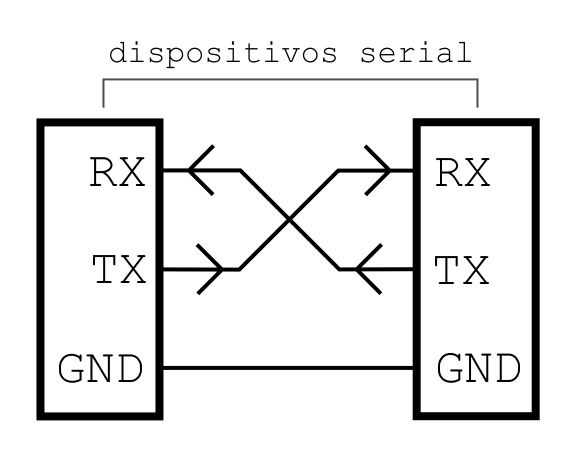
\includegraphics[scale=0.5]{figuras/cap2/serial.jpg}\\
  Fonte: Elaborada pelo autor.
  \label{serial}
  \end{center}
  \end{figure}


  A taxa de transmissão de dados é ajustável e definida em bits por segundo (baud) na função \textit{begin()}, onde podem ser empregadas as taxas recomendadas pelo fabricante (300, 600, 1200 etc) ou uma taxa específica para comunicação pelos pinos 0 e 1 com componentes que requeiram uma taxa de bits por segundo particular. Além disso, esses pinos podem ser usados para comunicação com dispositivos externos TTL serial conectando o pino RX do Arduino ao pino TX do dispositivo e o pino TX no RX do dispositivo.  

  Vale ressaltar que os pinos de comunicação serial do Arduino operam sob o padrão TTL e não podem ser conectados diretamente a uma porta serial RS-232, pois este padrão opera em nível de tensão $\pm 12$ V e pode danificar a placa. Desta forma, o \textit{hardware} serial envia e recebe dados na forma de pulsos elétricos que representam sequências de bits. Os zeros e uns que carregam a informação que compõe um byte podem ser representados de várias formas. No Arduino 0 volt representa um bit de valor \textbf{0} e 5 volts (ou 3.3 volts) representa um bit de valor \textbf{1}.

  Além dos padrões TTL e RS-232, existem outros protocolos de comunicação serial utilizados em aplicações de \textit{hardware}. O I$^{2}$C, por exemplo, é um padrão serial utilizado em componentes compatíveis com o Arduino, como módulos RTC (\textit{Real Time Clock}), módulo para \textit{display} LCD e chip expansor de portas. A seguir, o I$^{2}$C, juntamente com o TTL e o RS-232 são descritos sucintamente.

  \nomenclature{RTC}{Relógio de Tempo Real (\textit{Real Time Clock})}  

  \begin{itemize}
  \item{TTL} 
  
  O padrão que utiliza 0 volt para representar o bit 0 e 5 volts para o bit 1 é muito comum e conhecido como nível TTL, pois assim é como os sinais eram representados em uma das primeiras implementações de lógica digital, chamado de Lógica Transistor-Transistor (\textit{Transistor-Transistor Logic} -- TTL).
  Algumas placas têm um chip que converte a porta serial para o padrão USB, já aquelas que não dispõe de suporte para esse padrão, requerem um adaptador, que converte TTL para USB, para servir a conexão com um computador \cite{arduinocookbook}.
 
  
  \nomenclature{TTL}{Lógica Transistor-Transistor (\textit{Transistor-Transistor Logic})}
  
  \item{RS-232}
  
  O RS-232 é um antigo protocolo de comunicação que usa um nível de voltagem (+/- 12V) incompatível com os pinos digitais do Arduino -- por isso a necessidade do uso de um conversor RS-323/TTL  -- e normalmente tem nove pinos. A vantagem desse padrão sobre o TTL está na distância limite que ele alcança que é de 80 a 130 ft (pés) ou 24,384 a 39,624 metros, dependendo da taxa de bits e do tipo de cabo, enquanto que o USB chega a 16 ft ou 4,8768 m.


 \item{I$^{2}$C}
 
   Em projetos com Arduino, por exemplo, o Circuito Inter-integrado (\textit{Inter-Integrated Circuit} -- I$^{2}$C) é utilizado para tornar o circuito compacto, reduzindo a quantidade de fios e trilhas necessários para conectar os periféricos, como sensores, displays, teclados, leds, buzzers, etc, ou seja, todos aqueles dispositivos que utilizam pinos digitais para interagir com o microcontrolador. Caso esses dispositivos não sejam compatíveis com o I$^2$C, utilizam-se conversores ou chips que possibilitem a integração da tecnologia.
 
 \nomenclature{I$^{2}$C}{Circuito Inter-integrado (\textit{Inter-Integrated Circuit})}
 
   O I$^{2}$C é um barramento serial bidirecional desenvolvido pela Philips Semiconductors (agora NXP Semiconductors), usado para conectar periféricos de baixa velocidade a um computador, sistema embarcado ou celular. Esse barramento requer apenas duas vias para estabelecer a comunicação: uma via de dados serial (SDA - Seial Data) e uma via de clock serial (SCL - Serial Clock) \cite{i2c}. A Figura~\ref{i2c} mostra um exemplo de aplicação desse padrão.
 
 \begin{figure}[ht]
  \begin{center}
  \caption{Exemplo de aplicação I$^{2}$C.}
  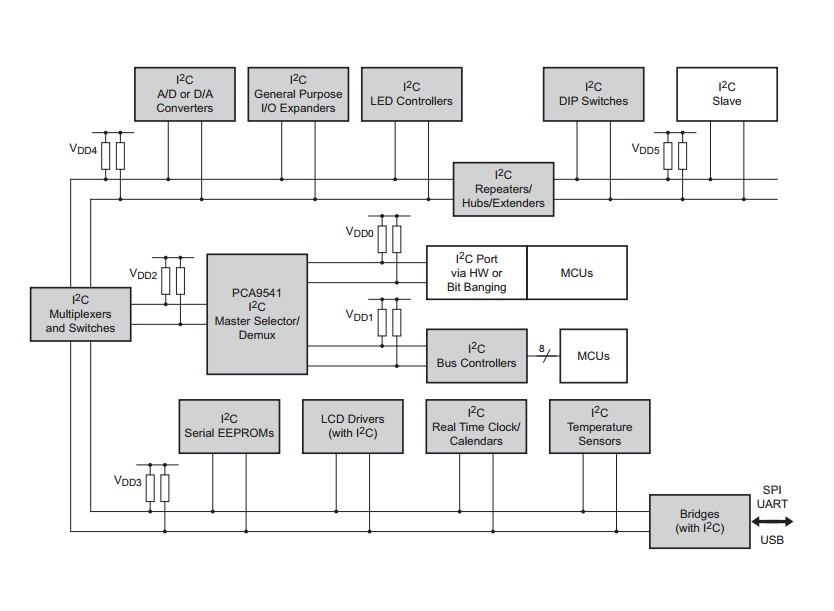
\includegraphics[scale=0.7]{figuras/cap2/i2c_app.jpg}\\
  Fonte: Adaptado de I$^{2}$C-bus specification and user manual\cite{i2c}.
  \label{i2c}
  \end{center}
  \end{figure}
  %\newpage
  
   A principal vantagem do uso desta tecnologia é que, por se tratar de um barramento multimestre, com apenas duas vias (dados e clock) é possível conectar vários dispositivos no mesmo barramento, cada um identificado por um endereço específico. O endereço atribuído a cada elemento no circuito normalmente é composto por 7 bits e isso dá um limite teórico de até 127 dispositivos em uma conexão \cite{arduinocc_i2c}. Além disso, eles podem ser configurados para receber ou transmitir dados e classificados como \textit{master} (mestre) ou \textit{slave} (escravo), onde o \textit{master} é o responsável por iniciar a comunicação e enviar informações a determinado \textit{slave} e este é encarregado somente por responder ao \textit{master}.
 \end{itemize}
 
 
 \section{Node.js}
 
   Apresentado em 2009 na JSConf Europa, por Ryan Dahl, o NodeJS é uma plataforma utilizada para a construção fácil e rápida de aplicações de rede escaláveis, em relação a outros programas de servidor como Apache ou o Tomcat.
   No lado do servidor, o Node funciona através da execução do V8 JavaScript. O V8 é um mecanismo subjacente da \textit{engine JavaScript open source}, um interpretador de alta performance escrito em C++, criado pela empresa de tecnologia Google que utiliza-o em seu navegador Chrome (no lado do cliente). No lado do cliente, a engine JavaScript interpreta e executa o código. Desta forma, é possível baixar o mecanismo e integrá-lo em qualquer aplicativo, pois ele não é restrito à execução em um navegador; o Node simplesmente usa esse mecanismo e o redireciona para uso no servidor.
 
   O principal destaque do Node é oferecer uma maneira mais fácil de criar aplicações de rede escalonáveis, pois o problema com os programas de servidor atuais, em linguagens como Java™ e PHP, é que a cada conexão feita no servidor é criada uma nova \textit{thread} que aloca 2 MB de memória. Nesse cenário, em um sistema com 8 GB de memória RAM, por exemplo, o número máximo teórico de conexões simultâneas fica limitado em torno de 4.000 usuários. Com o aumento do número de usuários seria necessário adicionar mais servidores, o que geraria mais custos operacionais e problemas técnicos. Assim, o Node busca solucionar esse problema criando um processo a cada conexão, o qual não requer a alocação de um novo espaço de memória, possibilitando o suporte a dezenas de milhares de conexões simultâneas. Ele aguarda eventos específicos, e quando um evento ocorre ele é respondido imediatamente. Enquanto um evento é processado, o Node não recusa qualquer outro pedido, ou seja, a resposta a outros eventos não depende que o atual seja concluído, os eventos são processados de forma que o primeiro que entra é o primeiro que sai em um \textit{event loop} \cite{nodejs, nodejs3}, como mostra a Figura~\ref{nodejs:eventloop}.  Assim, o modelo de programação do Node é orientado a eventos e apresenta uma sintaxe familiar, até para programadores iniciantes, que torna a implementação do \textit{software} mais fácil de codificar.
 
  \begin{figure}[!t]
  \begin{center}
  \caption{\textit{Event loop} do Node.js.}
  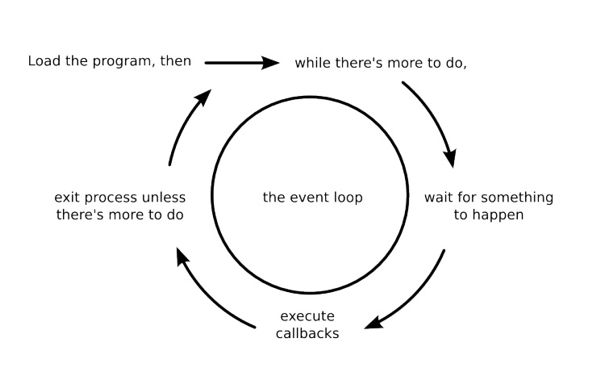
\includegraphics[scale=0.7]{figuras/cap2/nodejs_loop.jpg}\\
  Fonte: Adaptado de \cite{nodejs2}.
  \label{nodejs:eventloop}
  \end{center}
  \end{figure}
  %\newpage
 
   O Node é largamente empregado na construção de aplicações web. No entanto, a sua abrangência vai além de aplicações web, através do Node.js é possível escrever ferramentas de linha de comando, desenvolver aplicativos nativos para diferentes sistemas operacionais e construir aplicações \textit{desktop}. O Electron \cite{electron.atom}, por exemplo, é uma plataforma que permite a construção de apps desktop utilizando Node.js. Portanto, O Node é excelente para uma ampla gama de aplicações \cite{nodejs2}.

 
\section{SQL}
 
  SQL é uma linguagem de consulta estruturada de propósito especial usada para definir, acessar e manipular dados. É uma linguagem padrão universal para manipular banco de dados relacionais, além de ser não procedural, isto é, não é baseiada em sequências de prodedimentos/rotinas. 
 
 
 \section{MySQL}
 
  O MySQL é um sistema gerenciador de banco de dados relacional (SGBDR) gratuito e \textit{open source} que utiliza a linguagem SQL, sendo um dos mais populares do mundo. O MySQL é caracterizado pela sua rapidez, flexibilidade e segurança, além de ser relativamente simples~\cite{dubois2013}. 


\section{Placa de Circuito Impresso (PCB)}

  Um circuito impresso ou placa de circuito impresso (\textit{printed circuit board} -- PCB) consiste de um painel de material isolante, como Fenolite ou Fibra de Vidro, com uma fina camada de cobre condutor depositada sobre uma ou duas de suas faces através de um processo eletroquímico. As PCB's comuns, usadas em processos de confecção manual, podem ser de face única ou dupla, porém, as placas fabricadas em processos industriais, como placas de computador, celular ou outras produzidas em larga escala, são compostas de várias camadas de placas moldadas e integradas por meio de furos condutores. A camada de cobre sobre uma face constitui as trilhas condutoras que representam o circuito onde serão soldados e interligados os componentes eletrônicos. O processo de confecção de PCB's pode ser realizado empregando diversas técnicas existentes, sendo elas manuais ou industriais. O processo manual envolve algumas etapas fundamentais que são descritas a seguir \cite{pcb, pcb2}.

\nomenclature{PCB}{Placa de circuito impresso (\textit{Printed Circuit Board})}

\begin{enumerate}

\item \textbf{Projeto do circuito}

  Utilizando uma PCB virgem, um painel com face inteiramente coberta por camada de cobre, é feita a gravação de ``trilhas'' de cobre responsáveis por conectar os componentes de um circuito e substituir fios condutores. Em um processo manual, primeiramente, é necessário um \textit{software} de projeto de circuitos para desenhar as trilhas, como mostra a Figura~\ref{designcircuit}.


  \begin{figure}[ht]
  \begin{center}
  \caption{Design de circuito projetado no \textit{software} EAGLE 7.5.0 Light.}
  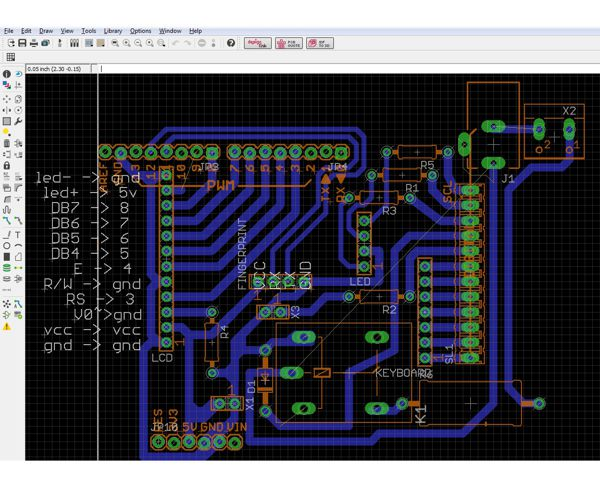
\includegraphics[scale=0.8]{figuras/cap2/designcircuit.jpg}\\
  Fonte: Elaborada pelo autor
  \label{designcircuit}
  \end{center}
  \end{figure}

  
  

\item \textbf{Impressão do design}
 
  A partir do layout do circuito mostrada na Figura~\ref{designcircuit}, é feita a impressão (Figura~\ref{impressdesigncircuit}) do design que representa o circuito, preferencialmente, em papel fotográfico para facilitar o processo térmico de transferência, e necessariamente em impressora a laser. 

  \begin{figure}[ht]
  \begin{center}
  \caption{Impressão do design do circuito para transferência.}
  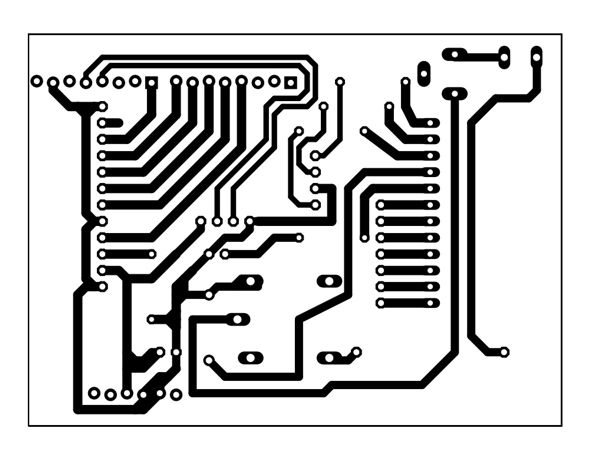
\includegraphics[scale=0.5]{figuras/cap2/impresscircuit.jpg}\\
  Fonte: Elaborada pelo autor
  \label{impressdesigncircuit}
  \end{center}
  \end{figure}
  


\item \textbf{Transferência} 

  De posse do design impresso, é feita a transferência da impressão para a placa virgem, normalmente, utilizando uma impressora de transferência térmica ou um ferro de passar roupas. Nesse processo, o toner presente no papel é termicamente transferido para a superfície de cobre da placa, assim, as regiões que representam o circuito cobrem a superfície de cobre da placa virgem, como mostra a Figura~\ref{designcircuit2}.

  \begin{figure}[!ht]
  \begin{center}
  \caption{Transferência do design impresso do circuito.}
  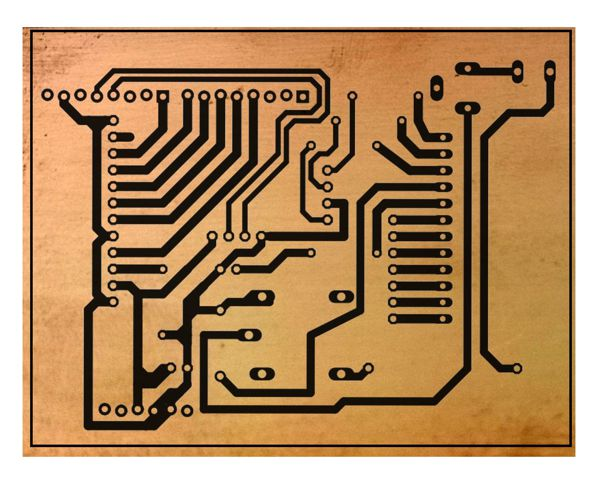
\includegraphics[scale=0.5]{figuras/cap2/impresscircuit2.jpg}\\
  Fonte: Elaborada pelo autor
  \label{designcircuit2}
  \end{center}
  \end{figure}





\item \textbf{Corrosão} 

  Nesta etapa deve ser feita a corrosão das regiões de cobre expostas, o que consiste em remover aquelas partes não cobertas por toner ou qualquer outro material que proteja e isole o cobre. O processo químico de corrosão ocorre utilizando-se soluções ácidas a partir de compostos químicos, como o Percloreto de Ferro ou outros, que em contato direto com o cobre reagem, retirando-o do painel de material isolante, deixando intactas apenas as regiões protegidas, ou seja, as trilhas do circuito, assim obtemos o resultado da Figura~\ref{designcircuit3}. O Cloreto Férrico ou Percloreto de Ferro, é um sal que em solução aquosa desenvolve ação corrosiva, e desta propriedade obtém-se marcações ou gravuras em metais \cite{gravuraemmetal}.

  \begin{figure}[!ht]
  \begin{center}
  \caption{Corrosão da superfície de cobre exposta.}
  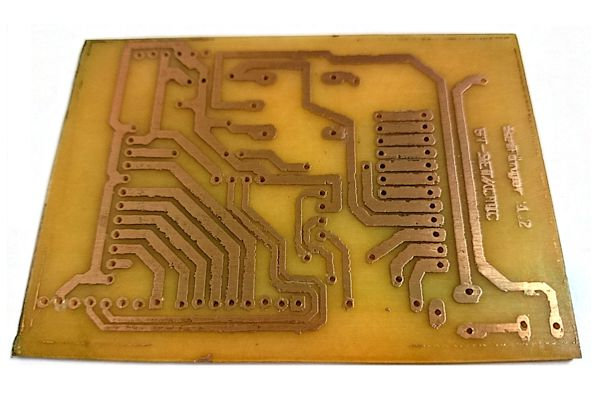
\includegraphics[scale=0.6]{figuras/cap2/impresscircuit3.jpg}\\
  Fonte: Elaborada pelo autor
  \label{designcircuit3}
  \end{center}
  \end{figure}



\item \textbf{Perfuração} 

  Após a gravação do layout do circuito na placa virgem é feita a sua furação nas respectivas ilhas de cobre, pontos onde os componentes serão conectados, utilizando um perfurador manual ou uma furadeira.

\item \textbf{Montagem e soldagem}

  Para finalizar, é feita a montagem e soldagem dos componentes em seus respectivos espaços na placa. Após está etapa, o circuito está pronto para testes e uso.


\end{enumerate}